\section{Auswertung}

\subsection{Apparatekonstanten}

\begin{itemize}
  \item Induktivität der Spule: $L = \SI{3,56(3)}{\milli \henry}$
  \item Kapazität des Kondensators: $C = \SI{5,015(15)}{\nano \farad}$
  \item kleinerer Widerstand: $R_1 = \SI{30,3(1)}{\ohm}$
  \item größerer Widerstand: $R_2 = \SI{271,6(3)}{\ohm}$
  \item Generatorwiderstand: $R_g = \SI{50}{\ohm}$
\end{itemize}

\subsection{Effektiver Widerstand und Abklingzeit}

Die aufgenommenen Messwerte befinden sich in Tabelle \ref{tab:effr}.

\begin{table}[H]
  \centering
  \caption{Messdaten}
  \label{tab:effr}
  \begin{tabular}{c S}
    \toprule
      {$U_C \:/\: \mathrm{V}$} & {$t \:/\: \mathrm{μs}$} \\
    \midrule
    4  &  17,8    \\
    32  &	 15,7   \\
    58  &	 14,1   \\
    86  &	 13,0   \\
    112  &	12,1  \\
    140  &	11,6  \\
    166  &	11,2  \\
    194  &	10,8  \\
    220  &	10,6  \\
    248  &	10,4  \\
    274  &	10,3  \\
    302  &	10,2  \\
    \bottomrule
  \end{tabular}
\end{table}
%
%\newpage
%
Aus diesen Messwerten folgt der Graph:

\begin{figure}[H]
  \centering
  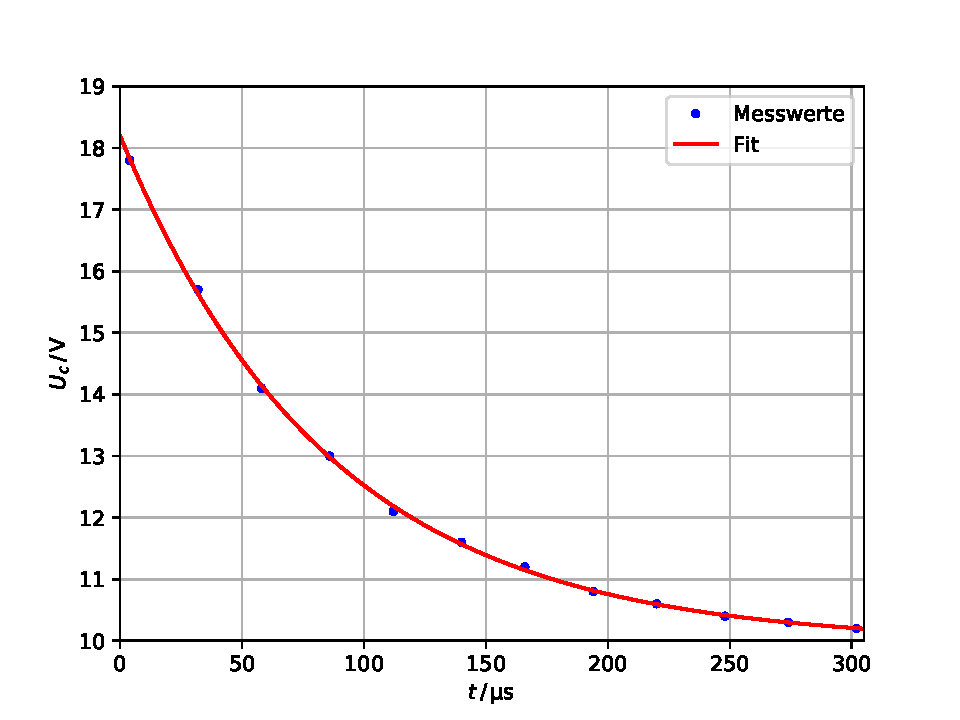
\includegraphics[width=\textwidth]{Plots/effr.pdf}
  \caption{$U_C$-$t$-Diagramm zur Bestimmung des effektiven Widerstandes und der Abklingzeit}
  \label{fig:effr}
\end{figure}

Mithilfe der Messwerte wird eine exponentiale Regression $a \cdot exp(-b) + c$ durchgeführt, die den Exponenten
$b = \SI{11684,87(19089)}{\Hz}$ liefert. Da $U \sim I$ gilt, folgt aus Gleichung \eqref{eqn:lsg}
\begin{align*}
    R_{\text{eff}} = \SI{82,50(152)}{\ohm} \\
    T_{\text{ex}} = \SI{85,58(140)}{\micro \second}
\end{align*}

Die Fehler erhält man aus der Gauß'schen Fehlerfortpflanzung
\begin{equation}
   \delta = \sqrt{ \sum_{i=1}^{n}(\frac{\partial y}{\partial x_i} \Delta x_i)^2}.
   \label{eqn:gaus}
 \end{equation}

Obwohl nur der kleinere Widerstand $R_1$ verwendet wurde, ist der effektive Widerstand
mehr als doppelt so groß. Dies lässt sich dadurch erklären, dass der Generatorwiderstand mit beachtet werden
muss. In den nachfolgenden Rechnungen wird immer der Gesamtwiderstand verwendet.

Der Theoriewert für den effektiven Widerstand ergibt sich aus
\begin{equation*}
  R_{\text{eff, theo}} = R_1 + R_g = \SI{80,3(1)}{\ohm},
\end{equation*}

während der Theoriewert für die Abklingzeit
\begin{equation*}
  T_{\text{ex, theo}} = \SI{87,92(76)}{\micro \second},
\end{equation*}

sich aus Gleichung \eqref{eqn:tex} bestimmen lässt.

\subsection{Aperiodischer Grenzfall}

Der experimentelle Wert für den Widerstand, bei dem der aperiodische Grenzfall eintritt
beträgt
\begin{equation*}
  R_{\text{ap}} = \SI{1290}{\ohm}.
\end{equation*}

Der Theoriewert
\begin{equation*}
  R_{\text{ap, theo}} = \SI{1677,96(71092)}{\ohm}
\end{equation*}

ergibt sich aus Gleichung \eqref{eqn:ap}.
\newpage
\subsection{Frequenzabhängigkeit der Spannung}

Die aufgenommenen Messwerte befinden sich in Tabelle \ref{tab:freq}.

\begin{table}[H]
  \centering
  \caption{Messwerte}
  \label{tab:freq}
  \begin{tabular}{c S}
    \toprule
      {$\nu \:/\: \mathrm{kHz}$} & {$U_C \:/\: \mathrm{V}$} \\
    \midrule
    15  &  11,0  \\
    20  &  11,8  \\
    25  &  13,3  \\
    30  &  15,6  \\
    31  &  16,2  \\
    32  &  16,7  \\
    33  &  17,3  \\
    34  &  17,6  \\
    35  &  17,8  \\
    36  &  17,8  \\
    37  &  17,6  \\
    38  &  17,2  \\
    39  &  16,6  \\
    40  &  15,8  \\
    45  &  12,4  \\
    50  &  10,2  \\
    55  &  8,8  \\
    \bottomrule
  \end{tabular}
\end{table}

Aus den Messwerten ergibt sich folgende Grafik:

\begin{figure}[H]
  \centering
  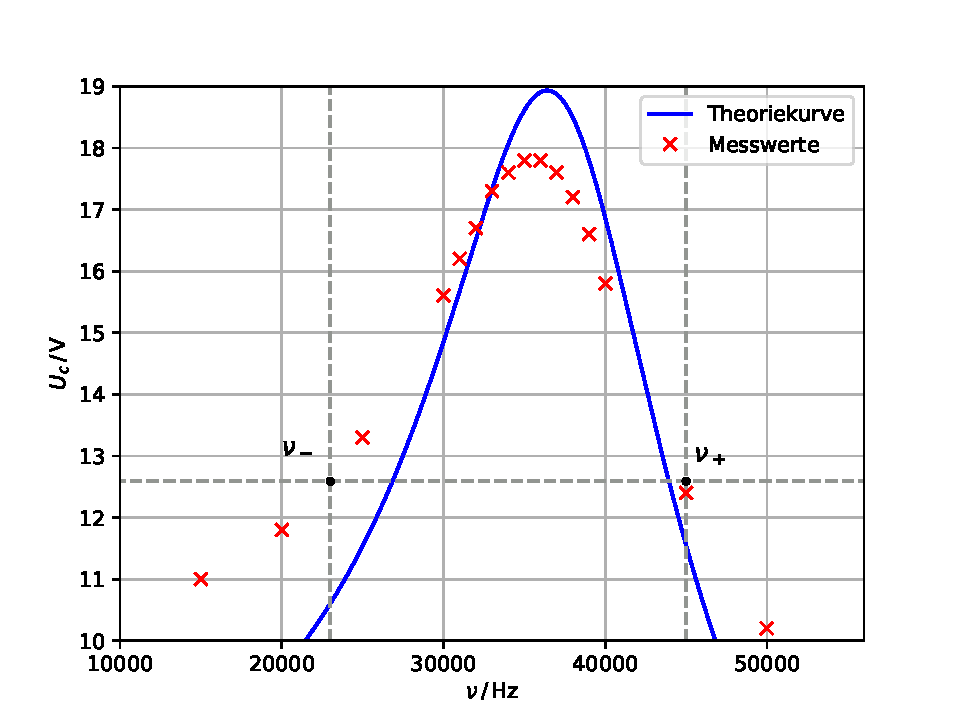
\includegraphics[width=\textwidth]{Plots/freq.pdf}
  \caption{$U_C$-$\nu$-Diagramm zur Bestimmung der Frequenzabhängigkeit der Spannung}
  \label{fig:freq}
\end{figure}

Die Güte des Schwingkreises ist damit
\begin{equation*}
  q = \SI{2,780(9)}{}.
\end{equation*}

Die Breite der Resonanzkurve beträgt nach Gleichung \eqref{eqn:bres}
\begin{equation*}
  \nu_+ - \nu_- = \SI{22000}{\Hz}.
\end{equation*}

Die Theoriewerte ergeben sich aus den Gleichungen \eqref{eqn:q}, \eqref{eqn:omega0} und \eqref{eqn:bres}:
\begin{align*}
  q_{\text{theo}} &= \SI{2,609(12)}{} \\
  (\nu_+ - \nu_-)_{\text{theo}} &= \SI{14499,78(12397)}{Hz}
\end{align*}

\subsection{Frequenzabhängigkeit der Phase}

Die aufgenommenen Messwerte befinden sich in Tabelle \ref{tab:phase}

\begin{table}[H]
  \centering
  \caption{Messdaten}
  \label{tab:phase}
  \begin{tabular}{c S}
    \toprule
    {$\nu \:/\: \mathrm{kHz}$} & {$a \:/\: \mathrm{μs}$} \\
    \midrule
    15  &  2,0  \\
    20  &  2,4  \\
    25  &  2,8  \\
    30  &  3,6  \\
    31  &  4,0  \\
    32  &  4,0  \\
    33  &  4,8  \\
    34  &  5,2  \\
    35  &  5,6  \\
    36  &  6,4  \\
    37  &  6,8  \\
    38  &  7,6  \\
    39  &  7,6  \\
    40  &  8,0  \\
    45  &  8,8  \\
    50  &  8,4  \\
    55  &  8,0  \\
    \bottomrule
  \end{tabular}
\end{table}

Die Phase berechnet sich aus:
\begin{equation}
  \Phi = \frac{a}{b} \cdot \SI{360}{°}.
\end{equation}

Dabei ist $b$ die Periodendauer der Generatorspannung,
die sich aus $b = \sfrac{1}{\nu}$ ergibt.
Daraus ergibt sich der Graph:

\begin{figure}[H]
  \centering
  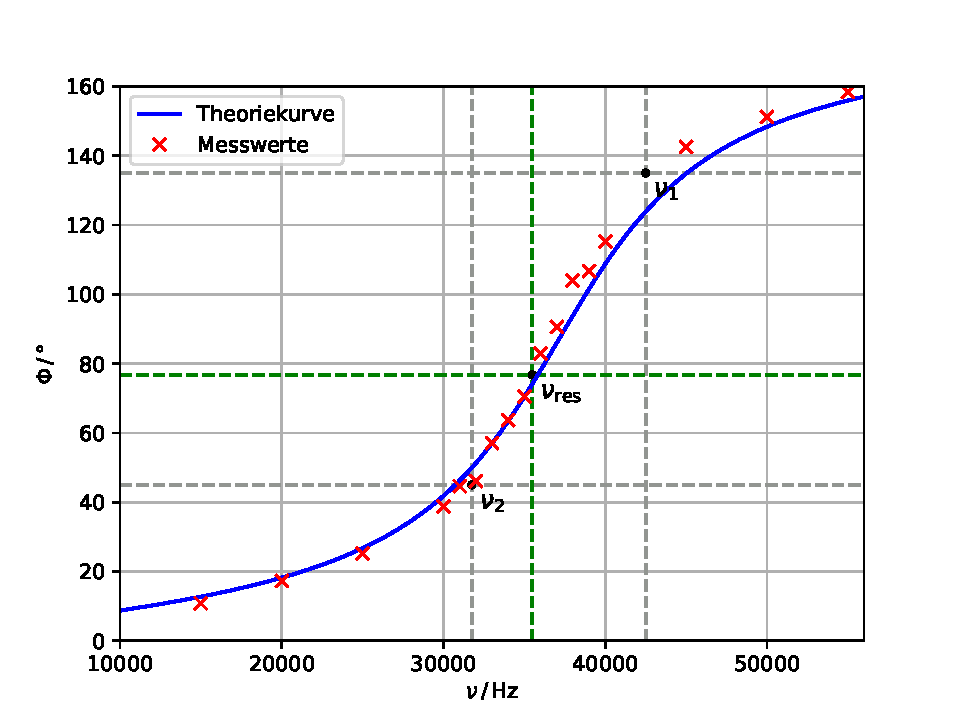
\includegraphics[width=\textwidth]{Plots/phase.pdf}
  \caption{$\Phi$-$\nu$-Diagramm zur Bestimmung der Frequenzabhängigkeit der Phase}
  \label{fig:phase}
\end{figure}

Die Resonanzfrequenz beträgt
\begin{equation*}
  \nu_\text{res} = \SI{35500}{\Hz}
\end{equation*}

und $\nu_1$ und $\nu_2$ sind
\begin{align*}
  \nu_1 &= \SI{42500}{\Hz} \\
  \nu_2 &= \SI{31750}{\Hz}
\end{align*}

Die Theoriewerte ergeben sich aus den Gleichungen \eqref{eqn:ores} und \eqref{eqn:omegas}:
\begin{align*}
  \nu_\text{res} &= \SI{36410,57(14248)}{\Hz} \\
  \nu_1 &= \SI{45765,00(715573)}{\Hz} \\
  \nu_2 &= \SI{31265,20(488738)}{\Hz}.
\end{align*}
